\documentclass[]{article}

% 1. Preamble and packages
\usepackage{amsfonts, amsmath, amssymb, amsbsy, amsthm}
\usepackage{graphicx}
\usepackage{epstopdf}
\usepackage{algorithmic}
\ifpdf%
  \DeclareGraphicsExtensions{.eps,.pdf,.png,.jpg}
\else
  \DeclareGraphicsExtensions{.eps}
\fi
\usepackage{amsopn}
\DeclareMathOperator{\diag}{diag}
\usepackage{booktabs}
\usepackage{bm}
\usepackage{todonotes}
\usepackage{caption}
\usepackage{float}
\usepackage{adjustbox}
\usepackage{multirow}
\usepackage{makecell}
\usepackage{tikz-cd}
\usepackage{subcaption} 

\newtheorem{lemma}{Lemma}
\newtheorem{rmk}{Remark}
\newtheorem{theorem}{Theorem}
\newtheorem{cor}{Corollary}
\newtheorem{definition}{Definition}

\DeclareCaptionType{equ}[Equation][List of Equations]
%\captionsetup[equ]{labelformat=empty}

% 1.5 Macros 
\newcommand{\R}{{\mathbb{R}}}
\newcommand{\bigOh}{\mathcal{O}}
\renewcommand{\vec}[1]{{{\mathbf{#1}}}}
\renewcommand{\t}{{\vec  t }}
\newcommand{\s}{{\vec  s}}
\renewcommand{\u}{{\vec  u }}
\renewcommand{\v}{{\vec  v }}
\newcommand{\f}{{\vec  f }}
\newcommand{\zero}{{\vec  0 }}
\newcommand{\A}{{A }}

\newcommand{\perm}{{ \tilde{A} }}

\newcommand{\off}{{E}}
\newcommand{\setoff}{{W}}
\newcommand{\lilpre}{{ \varphi }}
\newcommand{\bigpre}{{ \Phi }}
\newcommand{\precond}{{ M }}
\newcommand{\upleft}{{ V }}
\newcommand{\upright}{{ W }}
\newcommand{\lowright}{{ Q }}

\newcommand{\toediag}{{\lowright^D}}
\newcommand{\offd}{{\lowright^{LR}}}
\newcommand{\offoff}{{\lowright^{SN}}}
\newcommand{\smallsize}{{ s }}


\newcommand{\Schur}{{ B }}
\newcommand{\Hank}{{ H }}
\newcommand{\Toe}{{ L }}
\newcommand{\toe}{{ \ell }}
\newcommand{\toef}{{ \tilde{\toe}}}
\newcommand{\DST}{{ S }}
\newcommand{\Tau}{\mathcal{T}}




% 2. Paper title
\newcommand{\TheTitle}{%
  A Discrete-Sine-Transform based Preconditioner for Adaptive Meshes
}

% 2.5. Short title for running heads (if needed)
\newcommand{\TheShortTitle}{%
  \TheTitle
}

% 3. Student Name
\newcommand{\TheName}{%
 K. Wall
}

% 4. Student Address
\newcommand{\TheAddress}{%
  Tufts University,
  (\email{kate.wall@tufts.edu}, \url{https://katejeanw.github.io/}).
}

% 5. Acknowledge funding or other resources
\newcommand{\TheFunding}{%
  This material is based upon work supported by the National Science Foundation Graduate Research Fellowship under Grant No. 2234686
}

% 6. Collaborators, such as advisor or research collaborators
\newcommand{\TheCollaborators}{%
  James Adler,
  Xiaozhe Hu,
  Misha Kilmer
}

%% ---------------------------------------------
%% ---------------------------------------------
%\author{\TheName\thanks{\TheAddress}}
%\title{{\TheTitle}\thanks{\TheFunding}}
%\headers{\TheShortTitle}{\TheName}
%\ifpdf%
%\hypersetup{%
%  pdftitle={\TheTitle},
%  pdfauthor={\TheName}
%}
%\fi

\author{Kate Wall}
\title{A Discrete-Sine-Transform based Preconditioner for Adaptive Meshes}

\begin{document}

\maketitle

\begin{center}
In collaboration with:
  {\TheCollaborators}
\end{center}
\vspace{1cm}
% ---------------------------------------------
% ---------------------------------------------

\begin{abstract}
We present a preconditioner for solving fractional differential equations (FDEs) on an adaptive mesh. Adaptive refinement of the problem domain results in a stiffness matrix with Toeplitz blocks along the main diagonal, while the FDE yields a dense stiffness matrix where off-diagonal blocks are stored as low-rank approximations. Our adaptive preconditioner utilizes ideas from the circulant preconditioner of Chan and Strang [SIAM Journal on Scientific Computing, 1989] and the discrete-sine-transform based preconditioner of Bini and Di Benedetto [Association for Computing Machinery, 1990]. We take advantage of the Toeplitz blocks on the diagonal and accounts for the low-rank nature of the off-diagonal blocks. We demonstrate the adaptive preconditioner's effectiveness at accelerating convergence for our systems and emphasize its efficient application. This work presents theoretical results about the spectral clustering of the preconditioned system. In order to prove these results, special consideration is taken on how the low-rank blocks perturb the eigenvalues of the Toeplitz block-diagonal system. Numerical tests are used to inspect any assumptions and validate our results.
\end{abstract}

%
%\begin{keywords}
%  % 7. Keywords that describe the paper
%  Preconditioner, Adaptive Refinement, Finite-element Method, Toeplitz, Circulant, DST
%\end{keywords}


\section{Introduction} 
% Availabilitty of Xiaozhe's code / stiffness matrices 
In this paper we consider fractional differential equations \\ (FDEs) of the form 
\begin{equation}\label{FDE}
	D^{\alpha}_x u(x) = f(x), \ x \in (a,b),
\end{equation}
where $D^{\alpha}_x$ is the Riesz fractional derivative of order $1 < \alpha < 2$ and $f \in L^2([a,b])$. 


Fractional equations find applications in many fields such as fluid mechanics, electromagnetic fluids, image processing, and material science (see for example \cite{app_signals, app_electrom}). However, solving FDEs presents unique difficulties in numerical methods due to the non-locality of the operator resulting in a dense stiffness matrix, $A$. Additionally, as part of the fractional derivative the singular kernel, $k(x,s) = |x-s|^{1-\alpha}$, is integrated, resulting in end-point singularities which make Galerkin finite-element methods sub-optimal \cite{hierarch,superfast}. To address this, Jin and Zhou developed a reconstruction technique that isolates the singularity to improve finite-element method (FEM) convergence \cite{JZ}. Alternatively, Wang and Du developed a Toeplitz preconditioner that reduces iteration cost to $\bigOh(m \log m)$, where $m$ is the size of $A$, using the preconditioned conjugate gradient squared method \cite{superfast}. 

The above methods require uniform meshes. On a uniform mesh the FEM discretization results in a stiffness matrix that is Toeplitz. All methods on a uniform mesh leverage this structure for efficient linear solves. However, these methods fail to address high error near singularities, and instead the size of the mesh must grow. An optimal mesh would have the $L^{\infty}$ error equally distributed on each interval, but a uniform mesh does not, in general, satisfy this condition. Indeed, the singularities of FDEs force higher error in the intervals near the boundary and thus require very fine meshes to achieve uniform error below a given threshold. Alternatively, to achieve desired accuracy across the whole domain we use an adaptive mesh and adaptive finite-element method (AFEM) \cite{AFEM, Xiaozhe}. The usual AFEM algorithm iterates through the process 
\begin{equation} \label{AFEM}
	\texttt{SOLVE} \rightarrow \texttt{ESTIMATE} \rightarrow \texttt{MARK} \rightarrow \texttt{REFINE},
\end{equation} 
but the computational cost is dominated by the \texttt{SOLVE} step.

Zhao et al. used AFEM to solved FDEs using hierarchical matrices and geometric multigrid (GMG) \cite{Xiaozhe}. This method is done in $\bigOh(k N \log N)$ where $k$ is a parameter for low-rank approximations and $N$ is the degrees of freedom at the finest level. Numerical tests show this technique attains optimal convergence order, but there are no proofs guaranteeing such. Ainsworth and Glusa have detailed construction of the hierarchical representation in higher dimensions \cite{Glusa}.

In this paper, we construct a preconditioner, $\precond$, for the stiffness matrix, $\A$, from an AFEM discretization of Equation (\ref{FDE}). We show that the cost of solving the preconditioned linear system with a Krylov method is competitive with the GMG approach and furthermore prove that the preconditioned spectrum is clustered around 1, guaranteeing convergence. Our approach also has the advantage of avoiding hierarchical matrices and their sometimes cumbersome implementation. 

In the next section we present background information about structured matrices and preconditioning Toeplitz matrices. Then in Section (\ref{sec: precond}) we investigate what structure the adaptive mesh retains and how that is reflected in the structure of $\A$. We leverage this structure to apply preconditioning techniques formulated for Toeplitz matrices \cite{Chan_Strang, Chan_Yeung, precond_review, schrod}. This is followed by theoretical results about eigenvalue clustering of the preconditioned system in Section($\ref{sec: theory})$. Numerical results to validate any of our assumptions about the stiffness matrix and compare performance to the Zhao et al.'s GMG method are presented in Section (\ref{sec: numerical results}). 


% We leverage this idea to build a preconditioner for stiffness matrices generated from the adaptive finite-element method (AFEM) for FDEs. In this setting the problem is discretized on a nonuniform mesh, and the resulting stiffness matrix is dense. In the usual finite-element method (FEM) setting an uniform mesh results in a Toeplitz stiffness matrix. In the adaptive setting, after an initial solve on a uniform grid, the error on each element is estimated and the elements with largest error are refined via bisection. 

% application for FDEs
% similar systems result from mixed precision 
% These preconditioners can be thought of as coming from Kernels of displacement operators. Cite Kalaith and Chan-Yeung.

%We emphasize that our unique contributions are:
%\begin{itemize}
%	\item building circulant preconditioners for adaptive meshes 
%	\item proving the preconditioned system has eigenvalues clustered around 1
%	\item something else? numerical results? dealing with low-rank blocks?
%\end{itemize}

% overview of subsequent sections?

\section{Background} \label{sec: background}
\subsection{Properties of Structured Matrices}
\label{sec:matrix_props}
There has long been interest in solving Toeplitz linear systems efficiently. A matrix $A$ is called Toeplitz if $a_{ij} = a_{i-j}$. Arbitrary $n \times n$ matrices have up to $n^2$ entries and are solved directly in $\bigOh(n^3)$ FLOPS. Since a Toeplitz matrix has at most $2n-1$ unique entries, we expect to solve Toeplitz systems with $\bigOh (n^2)$ FLOPS, (see for example Levinson's algorithm, Trench's algorithm). Even with these improvements, however, fast Toeplitz algorithms are unstable in general and infeasible for large systems that arise in application \cite{stable}. Infinite or periodic Toeplitz matrices can be solved via a transformation to Fourier space and a discrete convolution in TODO time. On the other hand, finite Toeplitz systems are much more difficult to solve due to the boundaries of the mesh or matrix. To solve these systems, we turn to iterative Krylov and multigrid methods \cite{schrod, hierarch, Xiaozhe}. For these methods we take advantage of Toeplitz structure by using structured preconditioners. 

Toeplitz matrices commonly arise in partial differential equations discretization, FDEs, signal processing, and control theory. In application,  Toeplitz matrices are often symmetric positive definite (SPD) or symmetric positive semidefinite (SPSD). Given an SPD Toeplitz system $\Toe x = b$, the idea introduced by Strang in \cite{Strang_original} is to use a  circulant preconditioner, $C$, so that $C^{-1}Tx = C^{-1}b$ is solved in fewer iterations. 
A circulant matrix is a Toeplitz matrix, that additionally has the ``wrap-around'' property where the last entry of each row is the first entry of the subsequent row:
\begin{equ}[H]
	\begin{equation} 
		\Toe = \begin{pmatrix}
			\toe_0  &  \toe_{-1} & \cdots & \toe_{-(n-1)} \\
			\toe_{1} & \toe_0 & \cdots & \toe_{-(n-2)} \\
			\vdots & \vdots & \ddots & \vdots \\
			\toe_{n-1} & \toe_{n-2} & \cdots & \toe_0 
		\end{pmatrix} 
		\hspace{.15 in}
		C = \begin{pmatrix}
			c_0 & c_1 & \cdots & c_{n-1} \\
			c_{n-1} & c_0 & \cdots & c_{n-2} \\
			\vdots & \vdots & \ddots & \vdots \\
			c_{1} & c_{2} & \cdots & c_0 
		\end{pmatrix}.
	\end{equation}
	\caption{$\Toe$ is a Toeplitz matrix and $C$ is circulant.}
\end{equ}

As will be discussed in Section (\ref{stiffness}), the stiffness matrix resulting from AFEM applied to (\ref{FDE}) is not Toeplitz, but does contain SPD Toeplitz blocks. 
Toeplitz matrices have many special properties, here we focus on their connection to functions in the Wiener class. 
\begin{definition}[\cite{Chan_Strang}]
	Given a singly infinite, symmetric Toeplitz matrix $\Toe$ we define the finite subsection $\Toe_m$ to be the $m \times m$ principle submatrix. That is, 
	\begin{equation*}
		\Toe = \begin{pmatrix}
			\toe_0 & \toe_1 & \toe_2 & \\
			\toe_1 & \toe_0 & \toe_1 &  \ddots \\
			\toe_2 & \toe_1 & \toe_0 & \ddots  \\
			& \ddots & \ddots & \ddots  \\
		\end{pmatrix}
		\Toe_m = \begin{pmatrix}
			\toe_0 & \toe_1 & \cdots & \toe_{m-1} \\
			\toe_1 & \toe_0 & \cdots & \toe_{m-2} \\
			\vdots & \vdots & \ddots & \vdots \\
			\toe_{m-1} & \toe_{m-2} & \cdots & \toe_0 
		\end{pmatrix}.
	\end{equation*}
	Assume $\sum_{k=-\infty}^{\infty} |\toe_k| <\infty$, then the matrices induce functions $\toef(z) = \sum_{k=-\infty}^{\infty} \toe_k z^k$ and $\toef_n(z) = \sum_{k=-(n-1)}^{n-1} \toe_k z^k$ are real, positive, and in the Wiener class for $|z| = 1$.
\end{definition}

% Classical results on the eigenvalue distribution of Toeplitz matrices indicate that we cannot expect, in general, any clustering, and that the convergence of the method will be slow.
%% Toeplitz matrices and generating functions 

Previous work on Toeplitz systems offers many options for circulant preconditioners, (see \cite{precond_review}). Strang and R. Chan first proposed to construct a circulant $C$ by copying the central diagonals of $L$ into the required wrap-around entries. Assuming for simplicity $n = 2m$, then the first column of $C$ would be $\ell_0, \dots, \ell_m, \dots, \ell_0$ \cite{Chan_Strang}. Alternatively, Tony Chan constructed a circulant preconditioner, $C$, by averaging the diagonals of $L$. He shows this to be optimal in the sense that $||C-L||_F$ is minimal \cite{TChan}.

Although their construction differs, they are all diagonalized by some trigonometric transform matrix and are thus efficiently applied via the fast Fourier transform (FFT). The spectrum of the preconditioned systems are asymptotically the same \cite{precond_review}. In this paper the preconditioner we construct is based on the $\lilpre$ matrix class, introduced in \cite{Bini}. 
 

The $\lilpre$ preconditioner is not itself circulant, but is diagonalized by the type-I discrete sine transform (DST) matrix. Kailath and Olshevsky used a displacement operator kernel framework to unify the circulant preconditioners, $\lilpre$, and other preconditioners diagonalized by other discrete trigonometric matrices. Together these form a class of discrete-trigonometric-based preconditioners. Though our construction could be generalized to circulant preconditioners, we use $\lilpre$ because it does not require complex arithmetic needed for the FFT. 

\begin{definition} \label{tau_def}
Following \cite{Bini}, given a symmetric $n \times n$ Toeplitz matrix $\Toe$, we build a Hankel correction matrix, $H$, where 
\begin{align*}
	\Toe &= 
	\begin{pmatrix}
		\toe_0 & \toe_1 & \toe_2 & \cdots &\toe_{n-2}& \toe_{n-1} \\
		\toe_1 & \toe_0 & \toe_1 &  \cdots &\toe_{n-3}& \toe_{n-2} \\
		\toe_2 & \toe_1 & \toe_0 & \cdots &\toe_{n-4}& \toe_{n-3} \\
		\vdots & \vdots & \vdots & \ddots&\vdots & \vdots \\
		\toe_{n-2} & \toe_{n-3}   & \toe_{n-4} & \cdots &\toe_0 & \toe_1 \\
		\toe_{n-1} & \toe_{n-2}    & \toe_{n-3} & \cdots & \toe_1 & \toe_0 
	\end{pmatrix} 
	\\ \label{Hank}
	\Hank &= \begin{pmatrix}
		\toe_2 & \toe_3 & \toe_4 & \cdots & \toe_{n-1} & 0 & 0 \\
		\toe_3 & \toe_4 & \toe_5 & \cdots  & 0 & 0 & 0 \\
		\toe_4 & \toe_5 & \toe_6 & \cdots & 0 & 0 & \toe_{n-1} \\
		\vdots & \vdots & \vdots & \ddots & \vdots & \vdots & \vdots \\
		0 & 0 & 0 & \cdots & \toe_5 & \toe_4 & \toe_3 \\
		0 & 0 & \toe_{n-1} & \cdots & \toe_4 & \toe_3 & \toe_2
	\end{pmatrix}. 
	\end{align*}
	We can additionally define $\lilpre := \Toe - H. $
\end{definition}

Both $\Toe$ and $\Hank$ are symmetric, so they are completely represented by at most $n$ unique values: the diagonals of $\Toe: \toe_0, \toe_1, \dots, \toe_{n-1}$, and the anti-diagonals of $\Hank: \toe_2, \toe_3, \dots, \toe_{n-1},0,0 $. 
	
The following lemma summarizes properties of $\lilpre$.
\begin{lemma}[see \cite{Bini}] \label{lemma:tau}
	Let $\Toe$ be a Toeplitz matrix and $\Hank$ the corresponding Hankel correction as in Definition (\ref{tau_def}). Then $\lilpre = \Toe - \Hank$ has the following properties: 
\begin{enumerate}
	\item $\lilpre$ is diagonalized by the DST, $S$. We write $\lilpre = S \Lambda S^{-1} = S \Lambda S$.  
	\item $\lilpre$ can be applied in $\bigOh(n \log n)$ FLOPS.
	\item Let $\Toe_1$ be the first column of $\Toe$. Then, the $k$-th eigenvalue of $\lilpre$ is proportional to the $k$-th entry of $S\Toe_1$. Specifically, 
	\begin{equation} \label{eigs} \lambda_k(\lilpre) = c_k [S\Toe_1]_k, \ \text{where } c_k := \sqrt{\frac{n+1}{2}} \frac{1}{\sin(\frac{\pi k }{n+1})}.\end{equation}
	\item Each eigenvalue of $\lilpre$ is written as the truncated function $\toef_n$ evaluated somewhere on the unit circle, $\lambda_k(\lilpre) = \toef_n(z_k)$, where $|z_k| = 1$.
\end{enumerate}
\end{lemma}
% These preconditioner can also be thought of as coming from the kernel of a displacement operator. This framework is useful for generating yet other circulant preconditioners, (see \cite{Kailath}). 
% boundaries are the problem always (not infinite, block division)}
% Hankel matrices
% circulant and DFT/FFT (displacement kernel's)
% discrete convolution for exact solution and the boundary problem 

\subsection{AFEM stiffness matrix} \label{stiffness}
Again, let $\A$ be the stiffness matrix resulting from AFEM applied to (\ref{FDE}). During the $\texttt{MARK}$ module of AFEM (\ref{AFEM}), it is often the case that adjacent elements have similar error estimates, and are either both marked or both not marked for refinement. As a result, after several refinements there are still subsections of the domain that have been refined to the same level. We refer to these subdomains as \emph{locally uniform}.  Since uniform meshes give rise to SPD Toeplitz systems, wherever there are adjacent elements of the same size we find a corresponding Toeplitz block on the main diagonal of our stiffness matrix, $\A$. The size of this block depends on how many adjacent elements are the same size. In practice we have observed the greatest level of refinement is required near the boundary of the domain. In general we have larger Toeplitz blocks from locally uniform subdomains in the middle of the matrix, and smaller blocks near the boundary. At the extremes of the locally uniform intervals we always have interaction between elements of different sizes. This interaction means that Toeplitz blocks are never adjacent along the diagonal, instead there is at least one $1 \times 1$ `block' separating them. 

These $1 \times 1$ blocks, along with their corresponding rows and columns, can be viewed as additional boundaries imposed onto the system. As mentioned earlier, it is the boundaries of a Toeplitz system that necessitate more computation while solving, so we can anticipate that wise handling of these $1 \times 1$ block disruptions to the Toeplitz structure will be the key to making a good preconditioner. In order to better handle these $1 \times 1$ blocks, we solve the a permuted system, $\perm$, shifting the rows and columns associated with these blocks to the upper left corner of the matrix, constituting $V, W$ and $W^{\top}$, as shown in Figure (\ref{fig:perm}). Thus along the diagonal of the lower right block, $T$, remain Toeplitz blocks of size at least two. 

\begin{figure}[h]
	\centering
	\begin{tikzcd}
		PAP^{\top}  =  \tilde{A}  =  \begin{bmatrix} V & W \\ W^{\top} & \lowright \end{bmatrix}
	\end{tikzcd}
	\caption{The stiffness matrix $A$ is permuted and partitioned so that $\lowright$ contains all Toeplitz blocks along its diagonal. }
	\label{fig:perm}
\end{figure}

 Let $k$ denote the size of $\upleft$, that is the number of $1 \times 1$ blocks. It is natural to ask, and will indeed be important in constructing a preconditioner, how big is $k$ relative to $m = \text{size}(\A)$? It is difficult to get an exact handle on this theoretically, since it depends on how AFEM routines are implemented. However, in our numerical experiments we found that $k \approx \log(m)$ (see Section (\ref{validate})), and $k$ never grew faster than $m$. Let $p$ denote the number of Toeplitz blocks in $\lowright$. We might expect that $p$ is exactly one more than $k$. However, the adaptive refinement carried out in AFEM will occasionally create a few consecutive $1 \times 1$ blocks. So while we cannot guarantee an exact relationship between $k$ and $p$, it is true that $k \approx p$. 

% brief proof uniform mesh gives toeplitz?
% If the mesh is not fine enough to give the desired accuracy, one approach is to increase the number of elements, $n$. While this approach preserves uniformity, it usually requires recomputing the stiffness matrix entirely. Alternatively, if the level of refinement gives sufficiently small error for some parts of the domain, we can leave those unchanged and only refine in areas of larger error. This approach allows us to take advantage of computations that have already been performed, but the mesh is no longer uniform. 
%\todo[inline]{good spot to mention Toeplitz compression RNLA solvers?} 


\section{The Adaptive Preconditioner} \label{sec: precond} 
In this section we set forth the properties we require from a preconditioner. Using $\lilpre$ for its efficient inversion and good approximation of Toeplitz blocks, we construct our preconditioner, $\precond$, as an approximation to the LU decomposition of the permuted stiffness matrix.  

\subsection{Preconditioner Requirements} \label{sec: criteria}
A good preconditioner for an iterative method must in general decrease the total number of iterations, without increasing the cost of a single iteration. We borrow Kailath's \cite{Kailath} criteria for preconditioners, similar criteria is well-established in the literature (for example \cite{Bini}). 
\begin{enumerate} 
	\item Complexity of constructing and applying $\precond \in \R^{m \times m}$ should be $\bigOh (m \log m)$. \label{crit1}
	\item A linear system with $\precond$ should be solved in $ \bigOh (m \log m)$ operations. \label{crit2}
	\item The spectrum of $\precond^{-1} \perm$ should be clustered around 1. \label{crit3}
\end{enumerate}


\subsection{Constructing our Preconditioner}
\subsubsection{LU Decomposition of $\perm$}
To construct our preconditioner we must consider the permuted $1 \times 1$ blocks in $\upleft$ and the structured pieces of $\lowright$. 
Using the Schur complement, we can obtain a block-LU decomposition for our permuted stiffness matrix. It will be notationally convenient to define the Schur complement matrix $\Schur :=  \lowright - \upright^{\top} \upleft^{-1} \upright$. 
\begin{equation} \label{LU}
	\perm = LU = \begin{pmatrix}
		I & 0 \\ \upright^{\top} \upleft^{-1} & I
	\end{pmatrix} 
	\begin{pmatrix}
		\upleft & \upright \\ 0 & \Schur
	\end{pmatrix}
\end{equation}
It is straightforward to verify the inverses of the two factor matrices are,
\begin{align*}
	L^{-1} &= \begin{pmatrix}
		I & 0 \\ -\upright^{\top} \upleft^{-1} & I
	\end{pmatrix} \\
	U^{-1} &= \begin{pmatrix}
		\upleft^{-1} & -\upleft^{-1} \upright\Schur^{-1} \\ 0 & \Schur^{-1}
	\end{pmatrix}
\end{align*}

Recalling that $k = \text{size}(\upleft)$ is much smaller and slower-growing than $n$, inverting $\upleft$ will not contribute to our overall costs. Next, we can invert $\Schur$ using the Sherman-Woodbury-Morris formula, $\Schur^{-1} = \lowright^{-1} + \lowright^{-1}\upright^{\top}(\upleft-\upright\lowright^{-1}\upright^{\top})^{-1}\upright\lowright^{-1}$. Notice, however, it requires the prohibitively expensive inversion of $\lowright$. Here, we must leverage the Toeplitz blocks to build an adequate approximation to $\lowright^{-1}$. 


\subsubsection{Approximating  $\lowright^{-1}$}
Let $\Toe_1, \Toe_2, \dots, \Toe_p$ be the Toeplitz blocks ordered as they appear along the diagonal of $\toediag$, with respective sizes $m_1, m_2, \dots, m_p$. Then for each $\Toe_i$ we construct $\lilpre_i$ as in Definition (\ref{tau_def}). Stacking these blocks we build a block $\lilpre$ matrix as $\bigpre := \text{diag}(\lilpre_1, \lilpre_2, \dots, \lilpre_p)$. By application of Lemma \ref{lemma:tau} on each $\lilpre_i$, we can  apply $\bigpre^{-1}$ implicitly in $\bigOh \left( \sum_{j=1}^k m_j \log(m_j) \right) \leq \bigOh \left( k m \log ( m) \right) $,  where $m:= \max_j m_j$. Let $S_{m_i}$ denote the type-I DST matrix of size $m_i$.  Using Equation (\ref{eigs}) to calculate the eigenvalues of $\lilpre_i$, we write $\lilpre_i =  S_{m_i} \Lambda_i S_{m_i}$. 
\begin{equation} \label{diag}
	\bigpre^{-1} = 
	\begingroup % keep the change local
	\setlength\arraycolsep{3.5pt}
	\begin{pmatrix}
		S_{m_1} &&& \\ & S_{m_2} && \\ && \ddots & \\ &&& S_{m_p}
	\end{pmatrix}
	\begin{pmatrix}
		\Lambda_1^{-1} &&& \\ & \Lambda_2^{-1} && \\ && \ddots & \\ &&& \Lambda_p^{-1}
	\end{pmatrix}
	\begin{pmatrix}
		S_{m_1} &&& \\ & S_{m_2} && \\ && \ddots & \\ &&& S_{m_p}
	\end{pmatrix}.
	\endgroup
\end{equation}
The DST blocks in the outside matrices can be applied via the fast sine transform (FST) to do matrix multiplication in $\bigOh(m \log m)$ FLOPS. The eigenvalue matrix is diagonal and inverted in $m$ operations, and can be multiplied against a Toeplitz matrix embedded in a $2m \times 2m$ circulant matrix in $ \bigOh(m \log m)$ FLOPS. Moreover, both the FST and block arithmetic are highly parallelizable for more efficient implementation. This establishes Criteria (\ref{crit1}) and (\ref{crit2}) for $\bigpre$. Therefore $\bigpre^{-1}$ is fast to compute, and in Section (\ref{sec: theory}) we will show it is a good spectral approximation to $\lowright^{-1}$. 

\subsubsection{Defining the Adaptive Preconditioner, $\precond^{-1}$} \label{precond_def}
Let $\hat{\Schur} = \bigpre - \upright^{\top} \upleft^{-1}\upright$. Then define 
\begin{equation*}
	\hat{U} := \begin{pmatrix}
		\upleft & \upright \\ 0 & \hat{\Schur}
	\end{pmatrix}, \ 
	\hat{U}^{-1} =  \begin{pmatrix}
		\upleft^{-1} & -\upleft^{-1}\upright \hat{\Schur}^{-1} \\ 0 & \hat{\Schur}^{-1}
	\end{pmatrix}.
\end{equation*} 
Our preconditioner is given by 
\begin{align*}
	\precond^{-1} := \hat{U}^{-1} L^{-1} &= \begin{pmatrix}
		\upleft^{-1} & -\upleft^{-1}\upright \hat{\Schur}^{-1} \\ 0 & \hat{\Schur}^{-1}
	\end{pmatrix} \begin{pmatrix}
		I & 0 \\ -\upright^{\top}\upleft^{-1} & I
	\end{pmatrix} \\
	&= \begin{pmatrix}
		\upleft^{-1}  + \upleft^{-1} \upright\hat{\Schur}^{-1}\upright^{\top}\upleft^{-1} & -\upleft^{-1} \upright \hat{\Schur}^{-1} \\ -\hat{\Schur}^{-1}\upright^{\top}\upleft^{-1} & \hat{\Schur}^{-1} 
	\end{pmatrix}.
\end{align*}

The cost of applying $\precond^{-1}$ is dominated by application of the biggest block, $\hat{\Schur}^{-1}$. However, by using $\bigpre$ in place of $\lowright$, and consequently $\hat{\Schur}$ in place of $\Schur$, we use the Sherman-Morrison-Woodbury formula to calculate $\hat{\Schur}^{-1} = (\bigpre - \tilde{\upright^{\top}}\tilde{\upleft}^{-1}\tilde{\upright} )^{-1} = (\bigpre^{-1} + \bigpre^{-1}\upright^{\top}(\upleft-\upright\bigpre^{-1}\upright^{\top})^{-1}\upright\bigpre^{-1}$. Thus, using that fast application of $\bigpre$, as explained above, $\precond^{-1}$ can be applied in $\bigOh(m \log m)$ FLOPS. Therefore $\precond$ also satisfies Criteria (\ref{crit1}) and (\ref{crit2}). 


%The use of circulant preconditioners for Toeplitz systems originates from \cite{Chan_Strang}. Kailath showed how both Strang and Chan type preconditioners come from the kernel of displacement operators, they further detail eight specific preconditioners for each form of the discrete sine and cosine transforms. \todo[inline]{apply in n log n time}
%
%In our numerical results we use type TODO, discussed in \cite{Bini}. Though the results could be generalized to all eight forms. An important fact that we will use later:
%\todo[inline]{eigenvalues as points on function }




\section{Theoretical Results} \label{sec: theory}
% notation table ?
% 1x1 blocks consideration 
% Story: we know how this works on one block, what about block diagonal, what about with things happening outside of block diagonal? 
How tightly the eigenvalues cluster around 1 determines the speed of convergence. In this section we prove that the spectral clustering in criteria (\ref{crit3}) holds for $\precond$.  Proofs for clustering of discrete-trigonometric-transform based preconditioned problems in this area tend to follow a similar structure: show the preconditioned matrix can be written as the sum of the identity matrix, a small-norm matrix, and a low-rank matrix.  
The small-norm term has spectrum clustered around 0, forcing the clustering of the entire system around 1, with the number of outliers bounded by the rank of the low-rank term.

We build up to the clustering of the final preconditioned system in several steps. First, we briefly present our version of the spectral clustering proof for the case of $\lilpre$ acting on a single Toeplitz block. Then we expand this result to prove the clustering of $\bigpre^{-1}\lowright$; that is the block $\bigpre$ matrix applied to the Toeplitz blocks and corresponding off diagonal blocks of $\A_{22}$. Finally, we show how our handling of the $1 \times 1$ blocks preserves the spectral clustering of the whole system, $\precond^{-1} \perm$. 

%\begin{theorem}[Min-max Theorem]
%	Let $A \in \R^{n \times n}$ be symmetric with ordered spectrum $\lambda_1 \geq \cdots \geq \lambda_n$. Then 
%	\begin{align*}
%		\lambda_k &= \mathop{\max_{V \subset \R^{n \times n}}}_{\dim (V) = k} \ \mathop{\min_{x \in V}}_{x \ne \zero} \frac{(Ax,x)}{(x,x)} .
%	\end{align*} 
%\end{theorem}
%

%For convenience we state Weyl's Inequality and one other lemma that is useful to us later. Both these results are corollaries to the min-max theorem. 
%\begin{lemma}[Weyl's Inequality] \label{lemma:weyl} Let $M$ and $E$ be Hermitian $m \times m$ matrices. Then, for $A := M + E$ we have 
%	$$ | \lambda_k(A) - \lambda_k(M) | \leq ||E||_2 \ , 1 \leq k \leq m.$$
%	That is the eigenvalues of $A$ are at most $||E||_2$ away from the eigenvalues of $M$. 
%\end{lemma}

The following lemma will be of use to us throughout the section. 
\begin{lemma} \label{eig_lemma}
	Let $T \in \R^{n \times n}$ be an invertible matrix. Let $A \in \R^{n \times n}$, then $$\lambda_k(T^{-1}A) \leq \frac{\lambda_k(A)}{\lambda_{\min}(T)}.$$ 
\end{lemma}
\begin{proof}
	Using the min-max theorem, 
	\begin{align*}
		\lambda_k ( T^{-1} A) &= \min_{\dim V=k} \max_{x \in V} \left(  \frac{(Ax,x)}{(T x,x)}\right) \\
		&\leq   \min_{\dim V =k} \left[ \max_{x \in V} \left( \frac{(A x,x)}{(x,x)} \right)  \max_{x \in V} \left( \frac{(x,x)}{(T x,x)} \right) \right] \\
		&\leq \left[  \min_{\dim V =k}  \max_{x \in V} \left( \frac{(A x,x)}{(x,x)} \right)  \right] \max_{x \in \R^n} \left( \frac{(x,x)}{(T x,x)} \right)  \\
		&= \lambda_k(A)   \max_{x \in \R^n} \left( \frac{(x,x)}{(T x,x)} \right) \leq \lambda_k(A)  \frac{1}{\lambda_{\min}(T)}. 
	\end{align*}
\end{proof}

\subsection{Spectral Clustering of a Toeplitz Block} 
Proofs demonstrating the eigenvalue clustering of a circulant or trigonometric-based preconditioners on a Toeplitz matrices can follow a few strategies, here we briefly give our version, which utilizes the infinite matrix framework set forth in Section (\ref{sec:matrix_props}). Proofs in \cite{Bini} and \cite{Kailath} follow a similar technique, see \cite{Chan_Strang} for an approach relying on the infinite matrix framework and theory of collectively compact operators. In keeping with these proofs, we assume the generating function $\toef^{(i)}(z)$ induced by each Toeplitz block $\Toe_i$ is in the Wiener class and positive on the unit circle. That is, for all $1 \leq i \leq p, \toef^{(i)}(z) =  \sum_{j=-\infty}^{\infty} |\toe_j| <\infty$ and $\toe^{(i)}(z) > 0$ for $|z|=1$. 

\subsubsection{Approximating  $\lowright^{-1}$}
\begin{lemma}[Uniform positivity on the unit circle] \label{lemma: positive}
	Let $\Toe$ be a singly infinite, symmetric, Toeplitz matrix with diagonals $\toe_0, \toe_1, \dots$, and $\Toe_m$ is its $m \times m$ truncation. Assume the generating function $\toef(z)$ is in the Wiener class and positive on the unit circle. Then for $|z| = 1$, $\toef_m(z) > \varepsilon$ .
\end{lemma}
\begin{proof}
	Since $\toef(z) > 0$ for $|z|=1$, compactness of the unit circle implies that for some $\varepsilon > 0$, $\toef(z) > 2 \varepsilon$ for $|z|= 1$. By the Wiener class assumption, choose $N$ such that $\sum_{j=N}^{\infty} \toe_j z^j \leq \sum_{j=N}^{\infty} |\toe_j| < \varepsilon$. So for all $m \geq N$, 
	$$ 2 \varepsilon < \toe(z) = \toef_m(z) + \sum_{j=m}^{\infty} \toe_j z^j < \toef_m(z) + \varepsilon.$$
	% Thus $\toef_m(z) > \varepsilon$ on the unit circle. 
\end{proof}

\begin{lemma}[Eigenvalue Clustering on a Toeplitz Block, \cite{Bini, Kailath}] \label{block}
	Let $\Toe$, $\Toe_m$, $\toef$, and $\toef_m$ be as above, and 
	define $\lilpre$ as in \ref{tau_def}. Then for $m$ large enough, the spectrum of $\lilpre^{-1} \Toe$ is clustered around 1. 
\end{lemma}
\begin{proof}
Since $\lilpre = \Toe - \Hank$, 
$\lilpre^{-1} \Toe = \lilpre^{-1}(\lilpre + \Hank) =  I + \lilpre^{-1} \Hank $, it suffices to show that the eigenvalues of $\lilpre^{-1} \Hank$ are clustered around 0. 

We split the Hankel matrix into a low-rank and small-norm piece,  $\Hank = \Hank^{LR} + \Hank^{SN}$. Where $\Hank^{LR}$ contains the anti-diagonals $\toe_2, \dots, \toe_N$ with $s := \text{rank}(\Hank^{LR}) \ll m$. The small-norm descriptor is justified for $\Hank^{SN} = \Hank - \Hank^{LR}$, a Hermitian $m \times m$ matrix with at most two copies of $\toe_{N}, \dots, \toe_{m-1}$ in each row and column. Thus $||\Hank^{SN}||_2 = \sqrt{||\Hank^{SN}||_1 ||\Hank^{SN}||_{\infty}} = ||\Hank^{SN}||_1 < 2 \varepsilon$. Hence by Weyl's Inequality, the eigenvalues of $\Hank$ are clustered within $2 \varepsilon$ of zero with at most  $s$ outliers. 

Now by Lemma (\ref{eig_lemma}),
\begin{equation}  \label{eq:gen_bound}
	\lambda_k ( \lilpre^{-1} \Hank  ) \leq \lambda_k (\Hank)  \frac{1}{\lambda_{\min}(\lilpre )}  = \lambda_k (\Hank)  \frac{1}{\toef_m(z_{\min})} \leq \lambda_k (\Hank)  \frac{1}{\varepsilon}.
\end{equation}
Thus, the clustering of the spectrum of $\Hank$ around 0 implies the same for $\lilpre^{-1} \Hank$. 
\end{proof}
Equation (\ref{eq:gen_bound}) shows that the bigger $\lambda_{\min}(\lilpre)$, the stronger the bound. We can calculate this eigenvalue exactly using Lemma (\ref{lemma:tau}), and equation (\ref{eigs}). It can also be bounded in terms independent of $\lilpre$, using the generating function $\toef(z)$, as above. 

\subsection{Spectral Clustering of the Block System} \label{proof}
We now prove the spectral clustering of $\bigpre^{-1} \lowright$. 

\begin{figure}[h] 
	\centering
	\begin{tikzcd}[column sep=.005 in, row sep= 2pt]
		\adjincludegraphics[valign=c,width=.18\textwidth]{figures/A.png} & =  &\adjincludegraphics[valign=c,width=.18\textwidth]{figures/AD.png}   & + & \adjincludegraphics[valign=c,width=.18\textwidth]{figures/AE.png}  & + & \adjincludegraphics[valign=c,width=.18\textwidth]{figures/AF.png} \\
		\lowright && \toediag  &   & \offd &   & \offoff   
	\end{tikzcd}
	\caption{Illustration of the splitting of $\lowright$: $\toediag$ is block diagonal with Toeplitz blocks, blocks in $\offd$ are small and together form a low-rank matrix, and $\offoff$ is assumed to be small-norm due to weak interaction between elements.  }
	\label{fig:split}
\end{figure}

\begin{lemma} \label{lemma: block}
	Let $\A$ be the stiffness matrix as described in Section (\ref{stiffness}) and $\bigpre$ as described in Section (\ref{sec: precond}). Then the spectrum of $\bigpre^{-1} \lowright$ is clustered around 1. 
\end{lemma}

\begin{proof}
		It is easy to generalize the lemmas above to the block diagonal $\bigpre^{-1}$ acting only on the Toeplitz blocks, $\toediag$. The work in this proof is in showing that $\bigpre^{-1}(\offd  + \offoff)$ can also be split small-norm and low-rank pieces. 
		To begin we must further breakdown $\lowright$ into three summands, $\lowright = \toediag + \offd + \offoff$, where $\toediag$ contains the Toeplitz blocks, $\offd$ is low-rank ,and $\offoff$ is small-norm. 
	
	Due to the permutation, $\lowright$ has Toeplitz blocks of size at least 2 along its diagonal. We use $\toediag$ to denote the block diagonal with Toeplitz blocks. 
	
	The fractional derivative results in a dense matrix, but we observe off-diagonal decay, the strength of which depends on the fractional index $\alpha$. Elements sufficiently far from the diagonal are psychically separated and have weak interaction. However, merely excluding the Toeplitz blocks is not enough to get a small-norm matrix. As visualized in Figure (\ref{fig:split}), outside of the Toeplitz blocks, the entries closest to the diagonal occur at the boundary between Toeplitz blocks. We form small blocks from these adjacent-to-the-diagonal entries, comprising our low-rank term, $\offd$. The rank of which is bounded by the size of the block we take, $\smallsize$, times the number of blocks, which is the same as the number of $1 \times 1$ blocks, $k$. That is, $\text{rank}(\offd) \leq \smallsize k $. 
	Finally, the remaining entries makeup our small-norm matrix $\offoff$. We might naturally ask how big $\smallsize$ should be? The rank of $\offd$ contributes to the number of eigenvalue outliers, while the norm of $\offoff$ determines the strength of the clustering around 1. So a bigger $\smallsize$ would indicate more outliers but a tighter cluster, and a smaller $\smallsize$ indicates less outliers but a broader cluster. This is discussed more in Section (\ref{sec: numerical results}), but numerical tests indicate a good estimate for $\smallsize$ falls around 4. 
	
	Now we show the eigenvalues of $\bigpre^{-1} \lowright = \bigpre^{-1}(\toediag + \offd + \offoff)$ are clustered around 1. 
Let $\Hank$ be the block diagonal Hankel correction matrix, constructed as above but for each block in $\toediag$. Then that $ \toediag = \bigpre + \Hank$ we see that $\lowright = \bigpre + \Hank + \offd + \offoff$. So
\begin{equation} \label{eq: decomp1}
		\bigpre^{-1} \lowright  =
		 \bigpre^{-1}(\bigpre + H +\offd + \offoff) =
		 I + \bigpre^{-1}(H +  \offd + \offoff).
\end{equation}

%Our approach is to split $\Hank + \offd + \offoff$ into a small-norm term $\SN$ and a low-rank term $\LR$. Then
%Then it will suffice to show that the spectrum of $\bigpre^{-1}\SN$ is clustered around 0 and that $\bigpre^{-1}\LR$ contributes a bounded number of eigenvalue outliers. 

Splitting $\Hank$ is done via application of the splitting in the proof of Lemma (\ref{lemma: block}) to each block. As before, we have $\varepsilon > 0$ and choose $N_i$ smaller than each $m_i$ so that for every Toeplitz block the truncated function satisfies $a_{m_i} (z) > \varepsilon$ on the unit circle and $\sum_{i = N_i}^{\infty} |a_i| < \varepsilon$. 
Then $\Hank = \Hank^{LR} + \Hank ^{SN}$,  by separating into $\Hank^{LR}$ the anti-diagonals from block $i$ with coefficients $a_0, \dots, a_{N_i}$ and into $\Hank^{SN}$ the anti-diagonals comprising of $a_{N_i+1}, \dots a_{m_i}$ for each block. We note two important bounds: $||\Hank^{SN}||_2 < \varepsilon$ and $\text{rank}(\Hank^{LR}) \leq 2 p (N-1) $ where $p$ is the number of Toeplitz blocks and $N := \max_i N_i$. 
Equation (\ref{eq: decomp1}) can now be written as
\begin{equation}
	\bigpre^{-1} \lowright =   I + \bigpre^{-1}(\Hank^{LR}  + \offd)  + \bigpre^{-1}(\Hank^{SN} + \offoff). 
\end{equation}

This is ostensibly the low-rank plus small-norm representation we sought, but we finish the proof by giving explicit bounds on the rank and norm of these terms. 

Since $\bigpre$ is full-rank $\text{rank}(\bigpre^{-1} (\Hank^{LR}  + \offd)) = \text{rank}(\Hank^{LR}  + \offd)$. 
Now using each term's individual bounds, 
$$\text{rank}(H^{LR} + \offd) \leq \text{rank}(H^{LR}) + \text{rank}()\offd) \leq 2p(N-1) + \smallsize k. $$

It remains to show $ \bigpre^{-1} (\Hank^{SN} + \offoff) $ is small norm.
\begin{equation*}
		|| \bigpre^{-1} ( \Hank^{SN} + \offoff) ||_2  \leq 	|| \bigpre^{-1}  \Hank^{SN} ||_2 + 	|| \bigpre^{-1}  \offoff ||_2. 
\end{equation*}

The block multiplication $\bigpre^{-1} \Hank^{SN}$ is each $\lilpre$ acting on its corresponding Hankel correction. Since the matrices are SPD, $||\bigpre^{-1} \Hank^{SN}||_2 = \lambda_{\max} (\bigpre^{-1} \Hank^{SN}) \leq \frac{1}{\varepsilon} \lambda_{\max}(H)$, by Lemma (\ref{block}). 

Next, 
\begin{equation*}
	||\bigpre^{-1} \offoff||_2 \leq ||\bigpre^{-1}||_2 ||\offoff||_2 =\sigma_{\max}(\bigpre^{-1}) \sigma_{\max}(\offoff) = \frac{ \sigma_{\max}(\offoff)}{\lambda_{\min}(\bigpre)}.
\end{equation*}
Since $\offoff$ is small-norm this value is small. 

\begin{align*}
	|| \bigpre^{-1} ( \Hank^{SN} + \offoff) ||_2  &\leq 	|| \bigpre^{-1}  \Hank^{SN} ||_2 + 	|| \bigpre^{-1}  \offoff ||_2 \\
	& \leq \frac{1}{\varepsilon} \lambda_{\max}(H) +  \frac{ \sigma_{\max}(\offoff)}{\lambda_{\min}(\bigpre)}.
\end{align*}

%Since $\offd^{SN}$ made of blocks that have form $\sum_{i=r_{\offd}+1}^{n_{\offd}} \sigma_i \u_i \v_i*$ what can we say about $\lambda_k$?  
\end{proof}

The strength of this bound depends on $\lambda_{\min} (\bigpre)$, but can be written independently of $\bigpre$ in terms of the generating functions as in Equation (\ref{eq:gen_bound}). This dependence is the same for the single block case, and appears in similar proofs for discrete-trigonometric preconditioners (see for example \cite{Kailath}). 

In practice the block size, $m_i$, is determined by the AFEM algorithm, which in turn dictates the actual size $\varepsilon$ and hence the strength of clustering. Thus bigger Toeplitz blocks in $\A$ result in tighter eigenvalue clustering.
 
Notice that extending the proof from one Toeplitz block to the adaptive stiffness matrix relies only on being able to split the block into a small-norm and a low-rank piece. Thus, nothing about this proof is overly-specific to the $\lilpre$ preconditioner and the methods could easily be extended to the other types of circulant preconditioners given in \cite{Chan_Strang, Chan_Yeung}. 

% \todo[inline]{Lemma: summarize properties of $\bigpre$ like we did for $\lilpre$}
%\begin{lemma}
%	The adaptive preconditioner $\bigpre \in \R^{m \times m}$ has the following properties:
%	\begin{enumerate}
%		\item $\bigpre$ is block diagonalized by the type-I discrete sine transform (DST) blocks, see Equation (\ref{diag}).  
%		\item $\bigpre$ can be applied in $m \log m$ time.
%		\item The eigenvalues of $\bigpre^{-1} \A$ are clustered around 1. 
%	\end{enumerate}
%\end{lemma}


\subsection{Spectral Clustering of the Preconditioned System}
\begin{theorem}
	Following the established notation, 
	assume $\bigpre^{-1} ( \Hank^{SN} + \offoff)  < \varepsilon$ and define $s := \text{rank}(\bigpre^{-1} (\Hank^{LR}  + \offd))$. Then the spectrum of $\precond^{-1}A$ is clustered around 1, with at most $s$ outliers. 
\end{theorem}

%Assumption $\bigpre^{-1}\lowright = I + \varepsilon + N$, $N$ is low-rank 

\begin{proof}
Let $\Schur$ and $\hat{\Schur}$ be defined as in Section (\ref{precond_def}). By matrix multiplication and some simplification we get that the preconditioned system has the form:

\begin{align*}
	\precond^{-1} \perm &= \begin{pmatrix}
		\upleft^{-1}  + \upleft^{-1} \upright\hat{\Schur}^{-1}\upright^{\top}\upleft^{-1} & -\upleft^{-1} \upright \hat{\Schur}^{-1} \\ -\hat{\Schur}^{-1}\upright^{\top}\upleft^{-1} & \hat{\Schur}^{-1} 
	\end{pmatrix} \begin{pmatrix}
	\upleft & \upright \\ \upright^{\top} & \lowright
 	\end{pmatrix} \\
% 	&= \begin{pmatrix}
% 		I + \upleft^{-1} \upright\hat{\Schur}^{-1}\upright^{\top} -  \upleft^{-1} \upright\hat{\Schur}^{-1}\upright^{\top} & \upleft^{-1}\upright+\upleft^{-1}\upright \hat{\Schur}^{-1} \upright^{\top}\upleft^{-1}\upright - \upleft^{-1}\upright\hat{\Schur}^{-1}\lowright \\ 
% 		-\hat{\Schur}^{-1}\upright^{\top} + \hat{\Schur}^{-1}\upright^{\top} & -\hat{\Schur}^{-1}\upright^{\top}\upleft^{-1}\upright + \hat{\Schur}^{-1}\lowright
% 	\end{pmatrix} \\
 	&= \begin{pmatrix}
 		I & \upleft^{-1}\upright\hat{\Schur}^{-1}(\bigpre - \lowright) \\ 
 		0 & \hat{\Schur}^{-1}(\lowright-\upright^{\top}\upleft^{-1}\upright)
 	\end{pmatrix}.
\end{align*}
Since this is an upper-triangular system with a $k \times k$ identity block on the diagonal, we know that 1 is an eigenvalue of the preconditioned system, with algebraic multiplicity at least $k$, and the remaining $n-k$ eigenvalues are the spectrum of $\hat{\Schur}^{-1}(\lowright-\upright^{\top}\upleft^{-1}\upright)$. 

We examine this matrix block more closely. By the Sherman-Morrison-Woodbury formula $\hat{\Schur}^{-1} = (\bigpre - \tilde{\upright^{\top}}\tilde{\upleft}^{-1}\tilde{\upright} )^{-1} = (\bigpre^{-1} + \bigpre^{-1}\upright^{\top}(\upleft-\upright\bigpre^{-1}\upright^{\top})^{-1}\upright\bigpre^{-1}$, which we apply against $\lowright-\upright^{\top}\upleft^{-1}\upright$ to get 
\begin{align*}
\hat{\Schur}^{-1}(\lowright-\upright^{\top}\upleft^{-1}\upright) &= \bigpre^{-1}\lowright + \bigpre^{-1}\upright^{\top}(\upleft-\upright\bigpre^{-1}\upright^{\top})^{-1}\upright\bigpre^{-1}\lowright \\ &\ - \bigpre^{-1}\upright^{\top}\upleft^{-1}\upright  - \bigpre^{-1}\upright^{\top}(\upleft-\upright\bigpre^{-1}\upright^{\top})^{-1}\upright\bigpre^{-1}\upright^{\top}\upleft^{-1}\upright. 		
\end{align*}
We previously showed $\bigpre^{-1}\lowright = I + \bigpre^{-1} (\Hank^{SN} + \offoff)  + \bigpre^{-1} (\Hank^{LR}  + \offd)$, so now
\begin{align*}
	\hat{\Schur}^{-1}(\lowright-\upright^{\top}\upleft^{-1}\upright) &=  I +  \bigpre^{-1} (\Hank^{SN} + \offoff)  + \bigpre^{-1} (\Hank^{LR}  + \offd) \\ &\quad +  \big[   \bigpre^{-1}\upright^{\top}(\upleft-\upright\bigpre^{-1}\upright^{\top})^{-1}\upright  (I + \bigpre^{-1} (\Hank^{SN} + \offoff) + \bigpre^{-1} (\Hank^{LR}  + \offd)) \\
	&\quad - \bigpre^{-1}\upright^{\top}\upleft^{-1}\upright   -\bigpre^{-1}\upright^{\top}(\upleft-\upright\bigpre^{-1}\upright^{\top})^{-1} \upright \bigpre^{-1}\upright^{\top}\upleft^{-1}\upright  \big].
\end{align*}
We set aside the terms $I + \bigpre^{-1} ( \Hank^{SN} + \offoff)  + \bigpre^{-1} (\Hank^{LR}  + \offd) + ( \bigpre^{-1}\upright^{\top}(\upleft-\upright\bigpre^{-1}\upright^{\top})^{-1}\upright)( \bigpre^{-1} ( \Hank^{SN} + \offoff) + \bigpre^{-1} (\Hank^{LR}  + \offd))$, and show the remaining terms cancel out:
\begin{align*}
	& \bigpre^{-1}\upright^{\top}(\upleft-\upright\bigpre^{-1}\upright^{\top})^{-1}\upright - \bigpre^{-1}\upright^{\top}\upleft^{-1} \upright - \bigpre^{-1}\upright^{\top}(\upleft-\upright\bigpre^{-1}\upright^{\top})^{-1}\upright\bigpre^{-1}\upright^{\top}\upleft^{-1}\upright \\ 
	&=  [ - \bigpre^{-1}\upright^{\top}\upleft^{-1}  + \bigpre^{-1}\upright^{\top}(\upleft-\upright\bigpre^{-1}\upright^{\top})^{-1} (I - \upright\bigpre^{-1}\upright^{\top}\upleft^{-1})]\upright \\
	&= [ - \bigpre^{-1}\upright^{\top}\upleft^{-1}  + \bigpre^{-1}\upright^{\top}(\upleft-\upright\bigpre^{-1}\upright^{\top})^{-1} (\upleft - \upright\bigpre^{-1}\upright^{\top})\upleft^{-1}]\upright \\
	&= [ - \bigpre^{-1}\upright^{\top}\upleft^{-1}  + \bigpre^{-1}\upright^{\top}\upleft^{-1}]\upright = 0.
\end{align*} 

	
So the clustering depends on the spectrum of $I + \bigpre^{-1} (\Hank^{SN} + \offoff) + \bigpre^{-1} (\Hank^{LR}  + \offd) + ( \bigpre^{-1}\upright^{\top}(\upleft-\upright\bigpre^{-1}\upright^{\top})^{-1}\upright)(\bigpre^{-1} (\Hank^{SN} + \offoff) + \bigpre^{-1} (\Hank^{LR}  + \offd))$. Most of the non-identity terms here are easily characterized using the previous results as either low-rank or small-norm. However, we must assume $(\bigpre^{-1}\upright^{\top}(\upleft-\upright\bigpre^{-1}\upright^{\top})^{-1}\upright)\bigpre^{-1} (\Hank^{SN} + \offoff) $ is small-norm. Numerical validation of this assumption is found in Section (\ref{validate}). 
\end{proof}

We have now shown that $\precond$ satisfies all three criteria we sought in a preconditioner, as set forth in Section (\ref{sec: criteria}). 

\section{Numerical Results} \label{sec: numerical results}
To validate assumptions we made in our proofs and test the performance of our preconditioner, we ran tests to solve Equation (\ref{FDE}) with different right hand sides. We used preconditioned GMRES and solved to a tolerance of $\varepsilon = 10^{-7}$. In each case, we tested fractional indices $\alpha = 1.1, 1.2, \dots, 1.9$, paying special attention to $\alpha = 1.9$ since the condition number of the problem worsens as $\alpha$ approaches two. 

\subsection{Validating Assumptions}\label{validate}

\todo[inline]{
In building our preconditioner, we claimed that inverting $\upleft$ is relatively cheap since its size $k$, the number of $1 \times 1$ blocks , is smaller and grows more slowly than $m$. In pursuit of validating this assumption we must consider the mechanism by which AFEM refines the mesh. If AFEM is run to a set level of refinement, sufficient accuracy may be attained several levels before termination. Successive refinements will inflate $k$, with little return in improved accuracy. Thus to best measure how $k$ grows relative to $m$, we solved Equation (\ref{FDE}) with a known solution, $u(x) = 10x^2 (1-x^2)$ (see \cite{Xiaozhe} example 6.1 for more details) across values of $\alpha$, each time refining only until the $L^2$ error was below $\varepsilon = 10^{-7}$. }

\begin{figure}[h]
	\centering
	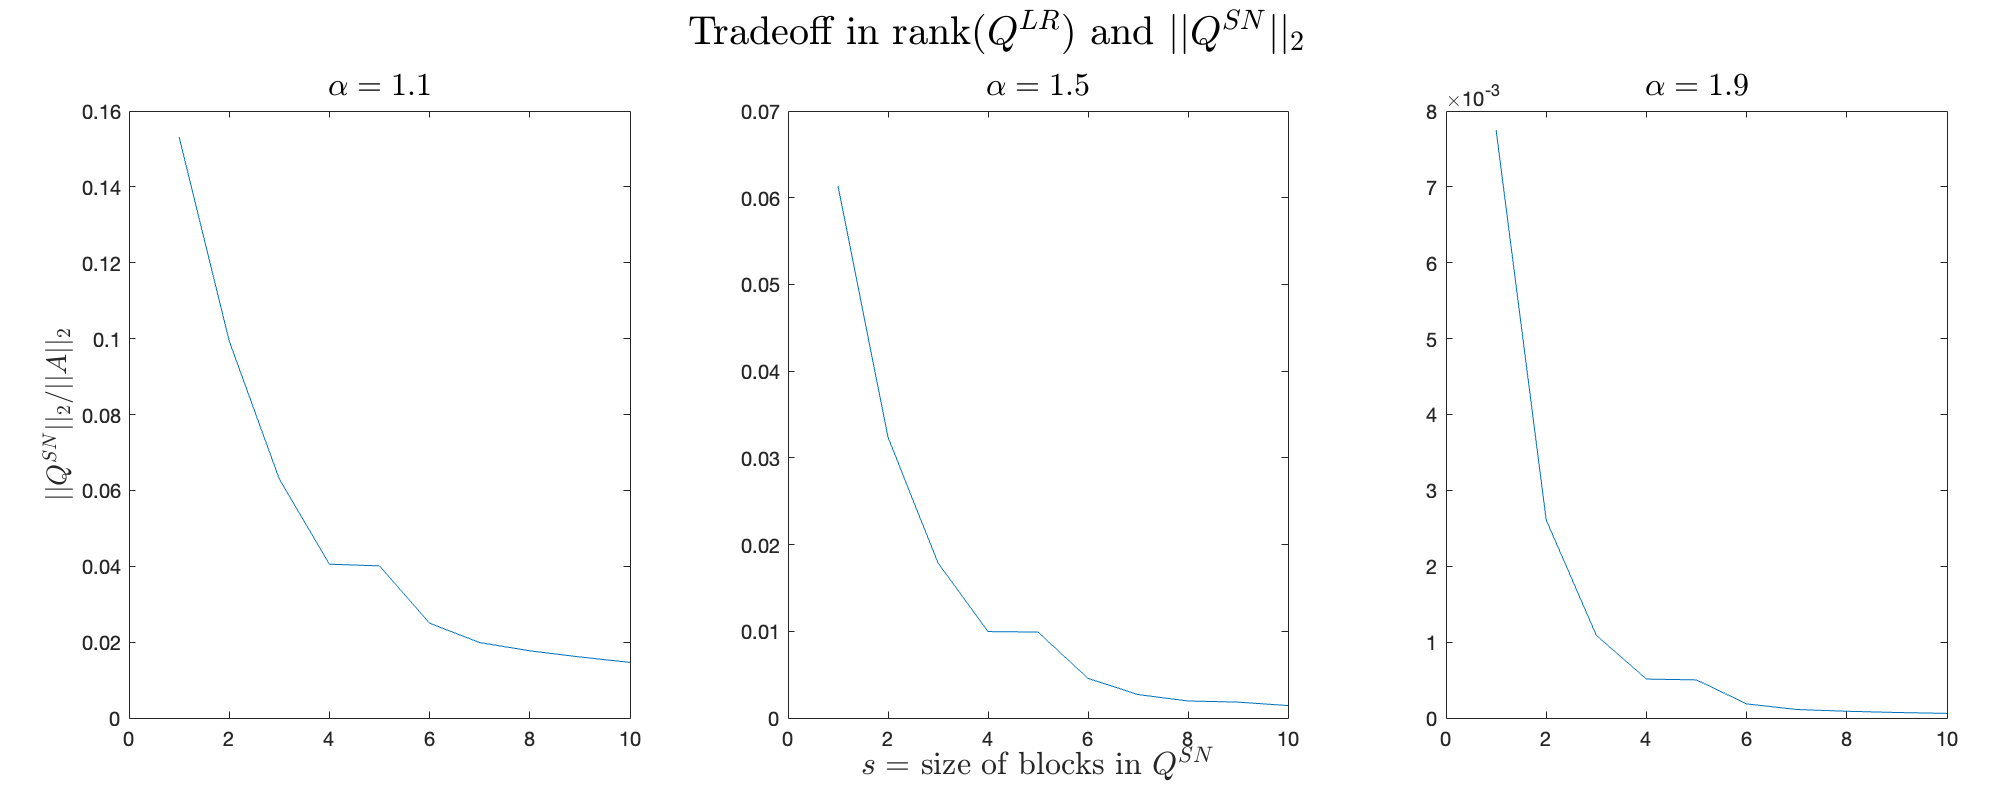
\includegraphics[width=  \textwidth]{figures/SN_vs_LR.png} \\
	\caption{The relative norm of $\offoff$ is plotted against $\smallsize$, the size of blocks in $\offd$. Initially, increasing $\smallsize$ drastically lowers $|| \offoff||_2$, but then levels off.}
	\label{fig:SN_vs_LR}
\end{figure}


In order to prove the spectral clustering, we made two assumptions about the structure of $\lowright$: the blocks adjacent to the diagonal are well-approximated by low-rank matrices and the other off-diagonal blocks are small-norm. The size of the blocks in $\offd$ has an inverse relationship to $|| \offoff||_2$.  The results in Figure (\ref{fig:SN_vs_LR}) visualize this relationship for solving Equation (\ref{FDE}) to a tolerance of $\varepsilon = 10^{-7}$, across various fractional indices, $\alpha$. The exact solution on this example is $u(x) = 10x^2 (1-x^2)$ (see \cite{Xiaozhe} example 6.1 for more details). Recall that $\text{rank}(\offd)$ bounds the number of outliers and $|| \offoff||_2$ relates to a bound on the clustering radius. We can interpret a larger $\smallsize$ as classifying more eigenvalues as outliers and a very tight cluster around 1, whereas a smaller $\smallsize$ and consequently larger $|| \offoff||_2$ would mean more eigenvalues are considered part of the cluster, but the cluster itself is bigger. This choice is a matter of interpretation for the theoretical proofs and not necessary for using the preconditioner, so it suffices to demonstrate that $\smallsize$ and $|| \offoff||_2$ can simultaneously be sufficiently small, as seen in Figure (\ref{fig:SN_vs_LR}). 


In our final step of the proof we assumed $(\bigpre^{-1}\upright^{\top}(\upleft-\upright\bigpre^{-1}\upright^{\top})^{-1}\upright)\bigpre^{-1} (\Hank^{SN} + \offoff) $ was small-norm. In the theoretical section we demonstrated that $||\Hank^{SN} + \offoff||_2$ is small, though it's exact value depends on how $\varepsilon$ is chosen in the proof of Lemma (\ref{lemma: block}). Here we demonstrate that the other part of this term, $||(\bigpre^{-1}\upright^{\top}(\upleft-\upright\bigpre^{-1}\upright^{\top})^{-1}\upright)\bigpre^{-1} ||_2$ is small. Example results of this value are given in Table (\ref{table: norm}).

\begin{table}[]
	\begin{tabular}{|c|c|c|c|c|c|c|c|c|}
	\hline
	Refinement  &&&&&&&& \\
	level &\thead{2}&\thead{3}&\thead{4}&\thead{5}&\thead{6}&\thead{7}&\thead{8}&\thead{9} \\
	\hline 
	$\alpha = 1.1$ & 1.42& 5.85& 3.86&	64.6&	32.137&	12.406&	28.14& N/A \\
	$\alpha = 1.2$ & 0.85&	6.31&	8.17&	95.9&	136.14&	66.526&	35.88& N/A \\
	$\alpha = 1.3$ & 0.55&	9.45&	5.19&	2.45	&24.142&	118.86&	76.59&	10.304  \\
	$\alpha = 1.4$ & 0.44&	2.25&	6.99&	1.51&	154.89&	95.706&	2.807&	2.474 \\
 	$\alpha = 1.5$ & 0.77&	0.91 &	1.57 &	10.085&	23.44157	&1.19&	1.270&16.43  \\
	$\alpha = 1.6$ & 0.39&	0.55&	0.46&	7.02&	25840.&	1.205&	1.936&	27.274 \\
	$\alpha = 1.7$ & 0.19	&0.50&	0.12&	0.419&	0.28575&	0.431&	137.48&	873.738 \\
	$\alpha = 1.8$ & 0.12&	0.10&	0.01&	0.011&	0.0261&	13.796&	1.345&	4152.50 \\
	$\alpha = 1.9$ & 0.01	&0.03	&0.00670&	0.00921	&0.01006&1.07&	0.05	&132.311 \\
	\hline
	\end{tabular}
	\caption{$||(\bigpre^{-1}\upright^{\top}(\upleft-\upright\bigpre^{-1}\upright^{\top})^{-1}\upright)\bigpre^{-1} ||_2$ for various $\alpha$, up to the refinement necessary for a solution with $L^2$ error below $\varepsilon = 10^{-7}$. Refinement level 1 is not included since it represents a uniform grid, where our preconditioner reduces to the Bini and de Benedetto preconditioner.}
	\label{table: norm}
\end{table}


\subsection{Performance Results}
\begin{figure}[h]
	\centering
	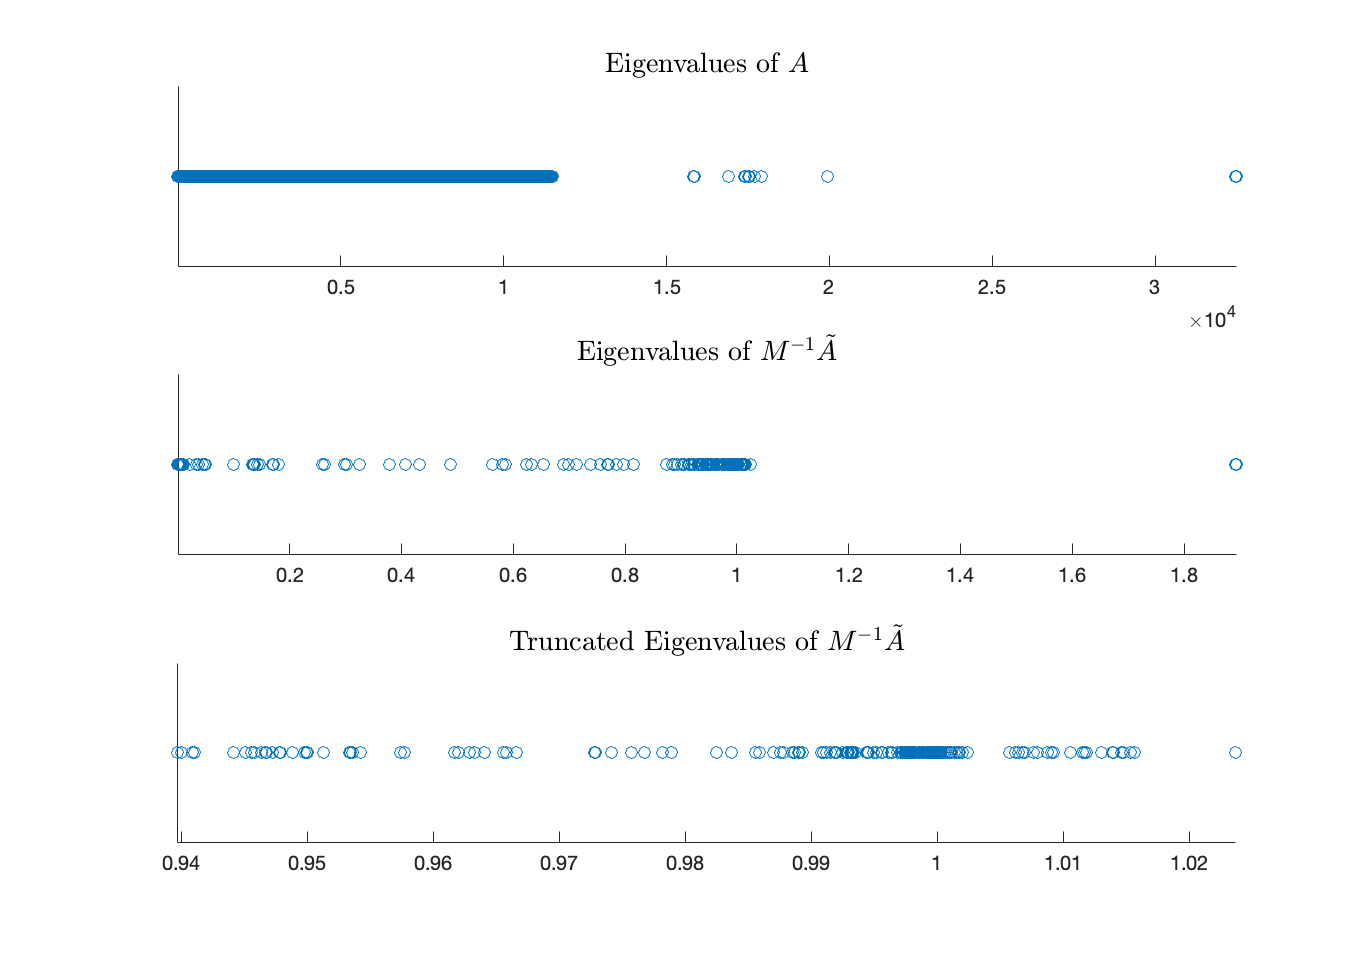
\includegraphics[width= \textwidth]{figures/eigs_4417_alpha9.png} \\
	\caption{Eigenvalue clustering before and after preconditioning for $m = 4417$ and $\alpha = 1.9$, notice the scale on the top plot. The bottom plot truncates the $p$ eigenvalues furthest from one, suggesting the number of Toeplitz blocks bounds the number of outliers in practice. }
	\label{fig:eigen_clusters}
\end{figure}


\begin{figure}
	\begin{subfigure}[h]{0.45\linewidth}
		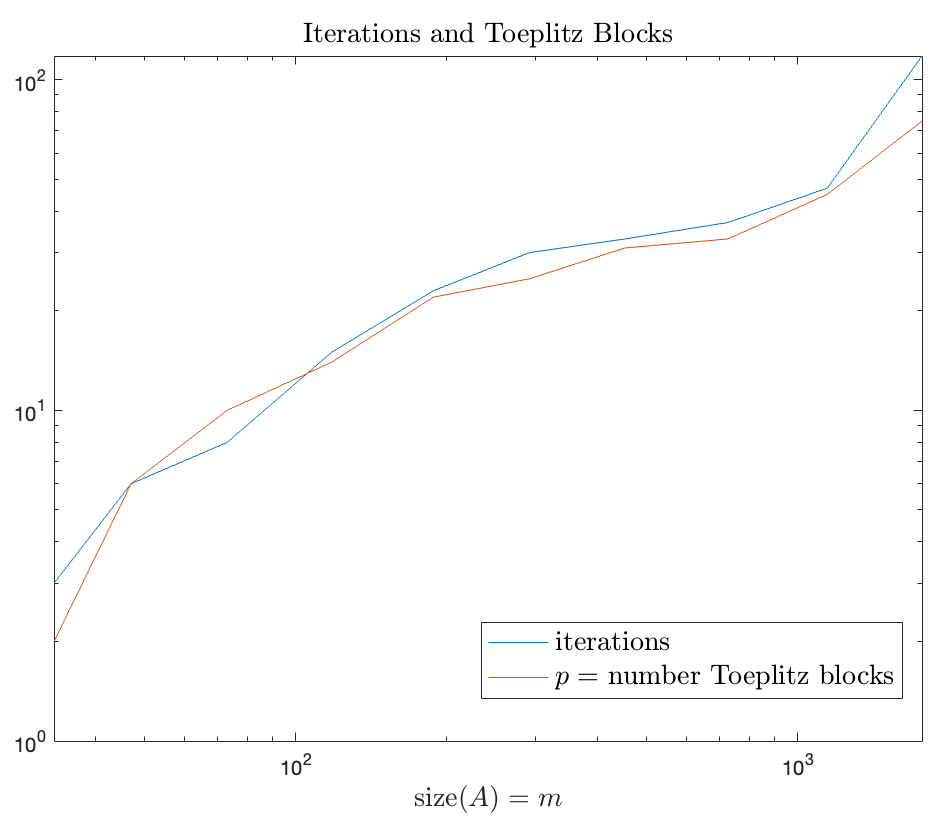
\includegraphics[width=\linewidth]{figures/iters_conv.png}
		\caption{Solving Equation (\ref{FDE}), where the exact solution is $u(x) = 10x^2 (1-x^2)$.}
	\end{subfigure}
	\hfill
	\begin{subfigure}[h]{0.45\linewidth}
		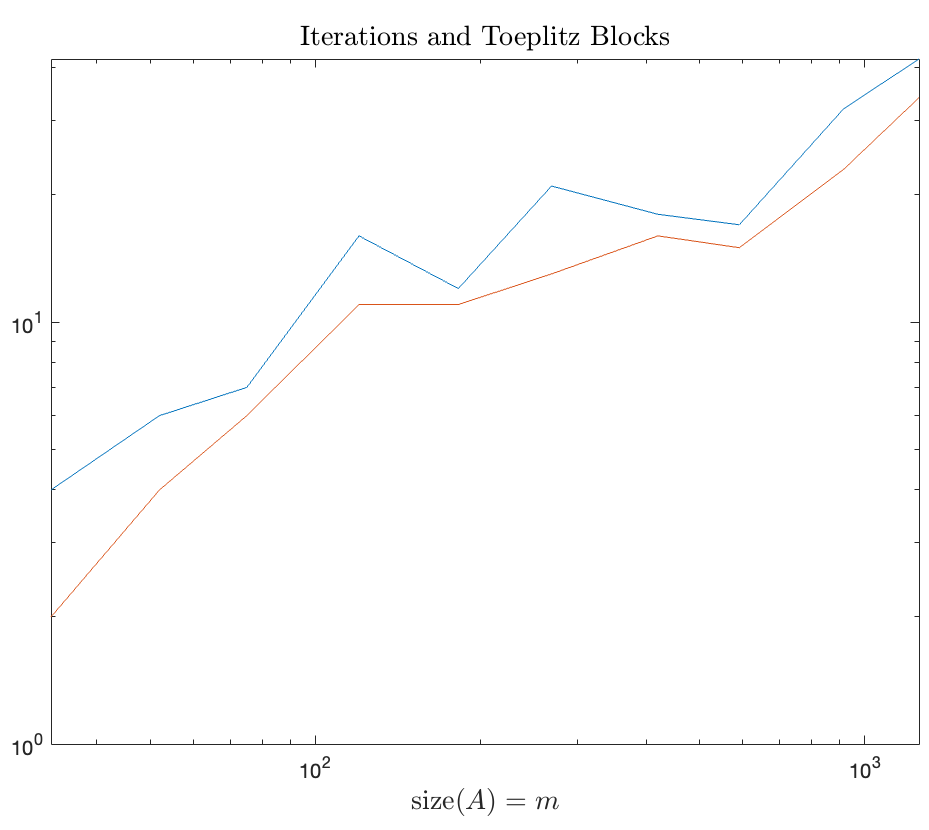
\includegraphics[width=\linewidth]{figures/iters_conv_ex2.png}
		\caption{Solving Equation (\ref{FDE}), with $f(x) = -(1+ \sin(x))$.}
	\end{subfigure}%
	\caption{Iterations to convergence below a tolerance of $\varepsilon = 10^{-7}$ for $\alpha = 1.9$, plotted with the number of Toeplitz blocks across increasing matrix size $m$. }
	\label{fig:conv}
\end{figure}

Example results of the spectrum before and after preconditioning are in Figure (\ref{fig:eigen_clusters}). These tests are for the problem (\ref{FDE}) with $\alpha = 1.9$ and exact solution $u(x) = 10x^2 (1-x^2)$ , as before. 
 Notice that although the proof allows for eigenvalue outliers far beyond the cluster, in practice everything remains within the interval $(0,2)$. 

Figure (\ref{fig:conv}) shows that the number of iterations required to converge closely follows the number of Toeplitz blocks in our stiffness matrix. Their approximate equality further supports the interpretation of $1 \times 1$ blocks acting as additional boundaries imposed on the problem, requiring roughly one iteration for each outlier eigenvalue these boundaries cause.

Finally, we compare our preconditioner to the hierarchical GMG method in \cite{Xiaozhe}. Figure (\ref{fig:L2_err}) shows that our estimated error closely follows that of the GMG method. 
\begin{figure}[h]
	\centering
	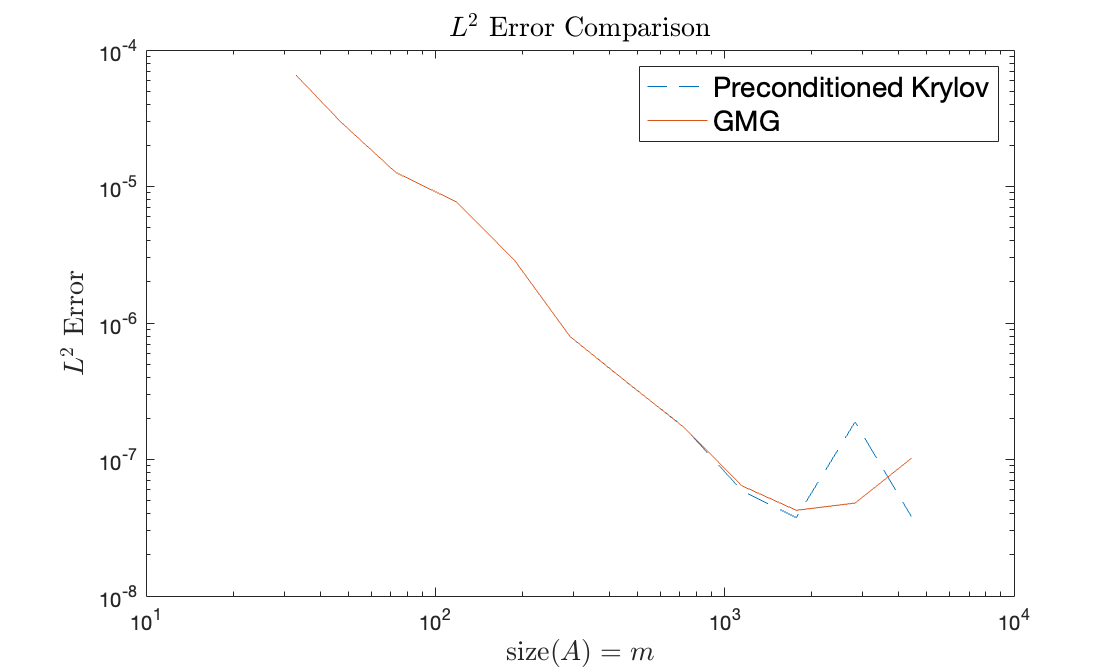
\includegraphics[width= .9\textwidth]{figures/L2_err.png} \\
	\caption{$L^2$ error comparison with Hierachical GMG method. }
	\label{fig:L2_err}
\end{figure}

\section{Conclusion}
The singularities inherent to FDEs require adaptive meshes to even approximately distribute error across intervals. The stiffness matrix resulting from AFEM is ill-conditioned. Previous work allows for hierarchical representation of $A$, enabling faster computation for solving with GMG \cite{Xiaozhe, Glusa}. We have offered an alternative approach, leveraging remaining structure in $A$ and utilizing well-known preconditioners for Toeplitz matrices. We have shown our preconditioner to be efficient to build, apply, and effective at reducing the number of Krylov iterations needed to solve the linear system. In numerical tests, we perform competitively against the GMG and additionally have theoretic proof of accelerated convergence. Future work could extend these ideas to FDEs in higher dimensions. 

% In the future, we will investigate how to customize the AFEM \texttt{MARK} module to build bigger Toeplitz blocks and thus get tighter clusters. 
\newpage
\bibliographystyle{siamplain}
\bibliography{references}

\end{document}
